\documentclass[12pt,aspectratio=169]{beamer}
\usetheme{iiasa}

\usepackage{ifthen}
\ifthenelse{\equal{\detokenize{notes}}{\jobname}}{%
\setbeameroption{show only notes}%
}{
%
}

\usepackage[
  maxnames = 1,
  style = authoryear,
  giveninits,
  terseinits,
  maxcitenames = 3,
  ]{biblatex}
\addbibresource{all.bib}

\usepackage{minted}
\usepackage[normalem]{ulem}

\title{‘Demand’ in MESSAGEix models}
\subtitle{Concepts, strategies, and examples}
\institute{Energy, Climate, and Environment (ECE) Program \\
  International Institute for Applied Systems Analysis (IIASA)}

\date{
  \texorpdfstring{MESSAGE Capacity Building Workshop — Wednesday, 12 June 2024}%
  {2024-06-12}}

\author{\texorpdfstring{Paul Natsuo Kishimoto\scriptsize\newline
  \href{mailto:paul.kishimoto@iiasa.ac.at}%
       {\ttfamily <paul.kishimoto@iiasa.ac.at>}}%
  {Paul Natsuo Kishimoto <paul.kishimoto@iiasa.ac.at>}}

\begin{document}

\maketitle

\begin{frame}
\frametitle{Intended outcomes}

At the end of this workshop session, learners should:

\begin{description}
  \item [distinguish] the \emph{background concept} of ‘demand’ from the specific meaning and function of the MESSAGE parameter \texttt{demand}.
  \item [understand] key choices to make when modeling demand, including:
    \begin{itemize}
      \item System of interest and its boundaries.
      \item Concrete measures, units of measure, and their meaning.
      \item How to obtain or project future values.
      \item How to handle other measures of interest.
    \end{itemize}
  \item [know] where to find additional examples, documentation, code, and data.
\end{description}

\end{frame}

\begin{frame}
\frametitle{What is ‘demand’?}
\framesubtitle{Let's begin with a definition from economics}

\pause
{\large “The amount of a good or service\footnote{collectively, ‘commodity’.} that consumers are willing to buy at a particular price.”}

\bigskip\pause
Dual to \structure{supply}: the amount that producers are willing to sell at a particular price.

\smallskip
These definitions assume a \structure{market} in which prices and quantities are determined, or at least some kind of \structure{exchange}, usually of money for the commodities.
\end{frame}
\note{
  We begin with the definition from economics, emphatically not because this is the only way to understand ‘demand’, but it's often what we have in mind as a \emph{background concept}.
}

\begin{frame}
\frametitle{How is ‘demand’ measured?}

Depends on the market and identity of the ‘consumers’ and ‘producers’:

\medskip
\begin{tabular}{rl}
  \structure{From the perspective of a…} & \structure{…“demand” is…} \\
  child's lemonade stand & \onslide<+->{glasses of lemonade} \\
  bicycle shop           & \onslide<+->{number of bicycles} \\
  laundromat             & \onslide<+->{loads of laundry washed} \\
  café                   & \onslide<+->{cups of coffee; croissants} \\
  public transit agency  & \onslide<+->{metro, tram, and/or bus trips provided} \\
  multinational oil firm & \onslide<+->{barrels of oil} \\
  mining company         & \onslide<+->{tonnes of material}
\end{tabular}

\medskip\pause
Measurements of demand are always \emph{simplifications}:
\begin{itemize}
  \item There is no such thing as “a bicycle”: there are thousands of specific models from hundreds of manufacturers, with different attributes.
  \item Producers and consumers are also heterogeneous.
\end{itemize}

\end{frame}

\begin{frame}
\frametitle{Modeling decisions: system boundaries}

Consider the “coffee machine” example model used in this workshop:

What goods and services did we choose \structure{\bfseries not} to include?

\medskip
\pause
{\footnotesize
\begin{itemize}
  \item Labour and materials (fertilizer) for growing beans.
  \item Transport of beans from plant to facility to roaster to point of sale.
  \item Packaging and retailing of beans.
  \item Manufacturing of coffee machines.
  \item Parts and raw materials for coffee machines.
  \item Production of electricity used by coffee machines.
  \item Alternative caffeine sources or other foodstuffs (hopefully) consumed by researchers.
\end{itemize}
(And yet we could—people do!—closely study ‘demand’ for any of these.)
}

\medskip\pause
\hspace{10mm}Usually ‘demand’ is near to, or crosses, our chosen system boundary.

\end{frame}

\begin{frame}
\frametitle{What is ‘demanded’ here?}
\framesubtitle{\href{https://mitpress.mit.edu/books/engineering-systems}{de Weck, Roos, Magee (2011) fig. 5.2, p.101}}

\includegraphics[
  width=\columnwidth,
  trim={0 485mm 0 0},
  clip]{de-weck-roos-magee-f5.2}
\end{frame}

\begin{frame}
\frametitle{What is ‘demanded’ here?}
\framesubtitle{\href{https://mitpress.mit.edu/books/engineering-systems}{de Weck, Roos, Magee (2011) fig. 5.2, p.101}}

\hspace{5mm}
\includegraphics[
  height=0.8\textheight,
  trim={0 242mm 0 178mm},
  clip]{de-weck-roos-magee-f5.2}
\end{frame}

\begin{frame}
\frametitle{What is ‘demanded’ here?}
\framesubtitle{\href{https://mitpress.mit.edu/books/engineering-systems}{de Weck, Roos, Magee (2011) fig. 5.2, p.101}}

\hspace{3mm}
\includegraphics[
  width=\columnwidth,
  trim={0 0 0 434mm},
  clip]{de-weck-roos-magee-f5.2}
\end{frame}

\begin{frame}
\frametitle{MESSAGE parameter $demand_{chlny}$}

As with other parts of the mathematical formulation: a \structure{highly abstract}/generic parameter, intended to be \structure{broadly applicable}.

\bigskip
Its values enter the \structure{constraints} named \texttt{COMMODITY\_BALANCE\_\{GT,LT\}}:
\begin{itemize}[<+->]
  \item These imply: “exactly «value [units]» of commodity $c$ \structure{must} be produced at level $l$, in node $n$, during time-slice $h$ of period $y$.”
  \item Any solution \structure{must} satisfy this constraint.
  \item Collective activity ($ACT$) of technologies $t \in T$ that directly $output$ to every $(c, h, l, n, y)$ \structure{must} equal the parameter value.
    \begin{itemize}
      \item Note that $ACT$ and $output$ have more dimensions (6 and 10) than $demand$ (5) → multiple possible solutions, some sub-optimal.
    \end{itemize}
  \item In turn, activity of ‘upstream’ technologies \structure{must} be sufficient for the $input$ of the above technologies (and so on).
\end{itemize}

\end{frame}

\begin{frame}
\frametitle{Modeling decisions: measure and unit}

To make use of the abstract $demand_{chlny}$ parameter, we must choose
which concrete \structure{measure}\footnote{Also ‘indicator’, ‘operationalization’.} (and \structure{units}) we will use to quantify the \structure{background concept}.

\bigskip
Example background concept: \structure{“transport demand”}

What concrete measures and units are chosen for which models?

\begin{description}
  \item [Base MESSAGEix-GLOBIOM] total “useful energy” [GW·a / year].
  \item [MESSAGEix-Transport] passenger-distance travelled (PDT) [km];

    freight volume [tonne-km].
  \item [Others (urban systems)] number of trips $[1]$.
  \item [Others (agent-based)] travel time $[\text{minutes}]$.
  \item [Others (economic, CGE)] expenditure on transport $[\text{EUR}]$.
\end{description}
\end{frame}

\begin{frame}
\frametitle{Background → concrete}

\begin{columns}
\column{0.5\paperwidth}
\includegraphics[height=0.78\textheight]{adcock-collier-2001_f1.png}

\column{0.4\paperwidth}
{\small \fullcite{adcock-collier-2001}}

\medskip
In practice, most of the conceptualization, operationalization, and measurement for the concepts we model \structure{has already been done} by other researchers.
\end{columns}
\end{frame}

\begin{frame}
\frametitle{Resolution and abstraction}

The \structure{scope} and \structure{resolution} of our model in \structure{time}, \structure{space} is determined \emph{by} our choice of \structure{units of analysis}\footnote{Not in this talk, but very important!} and \emph{in turn affects} the interpretation of our demand measures.

\bigskip
For example, having chosen PDT:
\begin{itemize}[<+(1)->]
  \item If one of our \texttt{node} set elements is "EU28", then our measure is:

  \structure{\emph{total} PDT \emph{for every person in the European Union}}

  …we are not modeling the PDT of \emph{any one particular individual}, or collection of individuals, or subgroups.

  \item If our \texttt{year} set includes \{2025, 2030, 2035\}, then our measure is:

  \structure{PDT \emph{in the representative year 2030 of the 5-year period named ‘2030’}}

  …even if we know the value will differ in the other years of the period, or from day to day or hour to hour within that year.
\end{itemize}
\end{frame}

\begin{frame}
\frametitle{Resolution and abstraction}
\framesubtitle{\href{https://mitpress.mit.edu/books/engineering-systems}{de Weck, Roos, Magee (2011) fig. 3.1, p.47}}

\centering
\includegraphics[height=0.78\textheight]{de-weck-roos-magee-f3.1}
\end{frame}

\begin{frame}
\frametitle{Data stages}
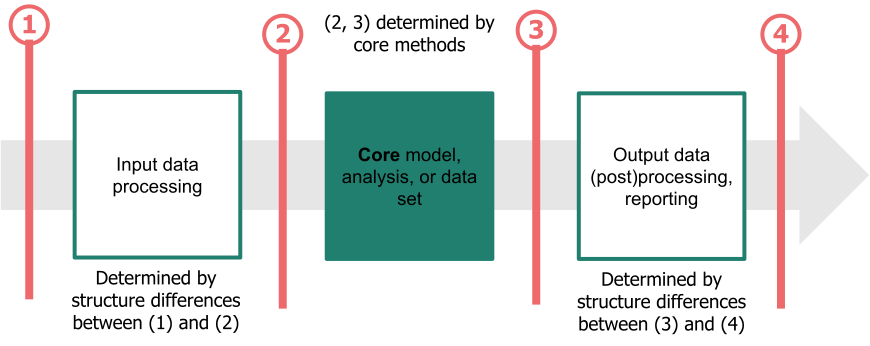
\includegraphics[width=\columnwidth]{data-stages}
\end{frame}

\begin{frame}
\frametitle{Modeling decisions: projections I}

The choice of \structure{time horizon} also leads us into a need for \structure{projected} demand.

\medskip
\begin{itemize}
  \item The model \emph{must} have $demand_{chlny}$ for \emph{every} $y$/period.%
    \footnote{If there is no value for a given period, there is nothing to be supplied,\\\hspace{25mm} and no technologies will be active.}
  \item The set $Y$ ($y \in Y$) in a MESSAGE model includes:
    \begin{enumerate}
      \item ‘Historical’ periods, before $y_0$.
      \item The “first model \sout{year} period”, or $y_0$.
      \item Future periods.
    \end{enumerate}
  \item Because we use an already-conceptualized measure, there is likely data available for (1) and likely (2) if it is before the present (usually a smart choice, for this reason).
\end{itemize}

\medskip
How then to obtain (3)?

\end{frame}

\begin{frame}
\frametitle{Modeling decisions: projections II}
For most measures we might choose as MESSAGE ‘demands’, there is a body of domain-specific methodology on projection. We either:

\bigskip
\begin{columns}[T]
\column{0.46\textwidth}
A) Find and use \structure{projections made by others}.
\begin{itemize}
  \item Best, when possible.
  \item Others probably made this their sole focus, rather than 1 model-building task among many → richer detail, more carefully-considered assumptions, validation.
  \item Easily described \& understood.
\end{itemize}

\column{0.46\textwidth}
B) \structure{Create our own projections} by \emph{ex ante} calculation (phase 1→2), using:
\begin{itemize}
  \item A separate model (simple or complex) in which our demand measure is the \emph{dependent variable}.
  \item \emph{Further} projections or assumptions for each of the independent variables in the model.
\end{itemize}

\end{columns}
\end{frame}

\begin{frame}
\frametitle{Modeling decisions: projections III}
Whichever method we choose, ask:

\bigskip
Do the projected data…

\smallskip
\begin{itemize}[<+->]
  \item …cover the entire \structure{time horizon} of our model?

  (If not: use option (B) for the remaining $y$; or shorten the horizon.)
  \item …use assumptions (such as socio-economic conditions: population, income, Gini; or policy) that are consistent with our model?
  \item …include \structure{alternate scenarios}?

  How do these align with scenarios we plan to implement in our model?
  \item …come with quantified uncertainty?
  \item …“bake-in” or duplicate phenomena that we plan to endogenize in our model?
\end{itemize}

\end{frame}



\begin{frame}
\frametitle{Modeling decisions: related measures}

If we select one measure of $demand$ but are \structure{also interested in other measures} (other systematized concepts, or related quantities) we must further decide:

\bigskip\pause
\begin{enumerate}[<+->]
  \item What \structure{relationship} do they bear to our chosen measure of $demand$?
  \item Is the relationship/related measure \structure{endogenous} to our model (“inside” our model; included in the optimal solution/output) or not (reporting; post-processing; \emph{ex ante} or \emph{ex post}).
  \item What \structure{input data} (assumptions or measurements) or \structure{data processing work} are needed to correctly parametrize (1)?
\end{enumerate}
\end{frame}

\begin{frame}
\frametitle{Data stages, again}
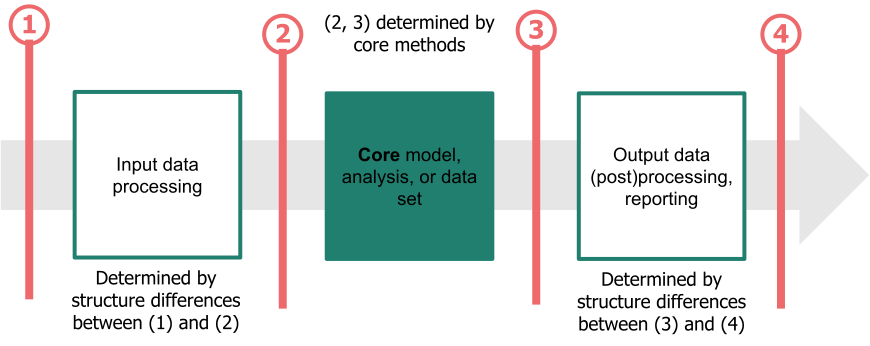
\includegraphics[width=\columnwidth]{data-stages}

Extra data (1) may enter the model (2) and/or be handled in the pre- (1→2) or post-solve (3→4) phases. In the latter case it may bypass the core entirely.
\end{frame}

\begin{frame}
\frametitle{Related measures: example 1}

Suppose we select \structure{trip count [\# of trips/dimensionless]} for the \texttt{demand} measure for \texttt{commodity} $c=\text{“transport”}$…

\pause
…but we are also interested in \structure{passenger distance travelled [km]}.

\bigskip
We answer the questions:
\begin{enumerate}[<+(1)->]
  \item What \structure{relationship} do they bear?
    \begin{itemize}
      \item Roughly $\text{trip count [trip]} \times \text{trip distance [km/trip]} = \text{PDT [km]}$.
    \end{itemize}
  \item Are these \structure{endogenous} or not?
    \begin{itemize}
      \item The model produces $c=\text{“transport”}$ to meet $demand$ specified as trip count. The solution is not affected by the PDT-equivalent. → Exogenous.
    \end{itemize}
  \item What \structure{input data and processing} are needed?
    \begin{itemize}
      \item We need data on \structure{trip distance [km]}.
      \item \emph{At least} a scalar, but \emph{up to} the dimensionality and resolution of $demand$.
      \item If the resolution/scale on any dimension is not matched, we must adapt.
    \end{itemize}
\end{enumerate}
\end{frame}

\begin{frame}
\frametitle{Related measures: example 2}

Suppose we select \structure{trip count [\# of trips/dimensionless]} for the \texttt{demand} measure for \texttt{commodity} $c=\text{“transport”}$…

\pause
…but we are also interested in \structure{final energy use [GJ]}.

\bigskip
We answer the questions:
\begin{enumerate}[<+(1)->]
  \item What \structure{relationship} do they bear?
    \begin{itemize}
      \item $\text{trip count [trip]} \times \text{energy intensity of a trip [GJ/trip]} = \text{final energy [GJ]}$.
    \end{itemize}
  \item Are these \structure{endogenous} or not?
    \begin{itemize}
      \item The technologies $t$ in our model that produce $c=\text{“transport”}$ also take $input$ measured as final energy [GJ] → Endogenous.
    \end{itemize}
  \item What \structure{input data and processing} are needed?
    \begin{itemize}
      \item We have likely already parametrized this in building our model.
      \item However we may need to transform, aggregate, etc. $ACT$ or others in our \structure{reporting} workflow to get precisely the quantity we want.
    \end{itemize}
\end{enumerate}
\end{frame}

\begin{frame}
\frametitle{Wrapping up}

Modeling ‘demand’ is much like other parts of model building:
\begin{enumerate}
  \item Move from a vague background concept/notion to a precise and complete description of what you will model.
  \item Implement that specification using features provided by MESSAGE.
\end{enumerate}

\bigskip
The remainder of the workshop has been focused on (2).

\smallskip
This session provided a sketch of how to do (1), and some basic examples.

\end{frame}

\begin{frame}
\frametitle{Learn more}
In order to address a wide range of research questions, IIASA ECE Program colleagues \& collaborators model a variety of ‘demands’ in different MESSAGEix-GLOBIOM \structure{variants}.\footnote{model versions with added detail or tailored modifications.}

\bigskip
Read the documentation/papers for these model variants and note how the above decisions were made:

\begin{description}
  \item [base MESSAGEix-GLOBIOM] “useful energy” [GW·a] for aggregate sectors.
  \item [MESSAGEix-Nexus] urban/rural drinking water; water for irrigation [$\text{km}^3 / \text{a}$].
  \item [MESSAGEix-Materials] amounts of raw and processed materials [tonne].
  \item [MESSAGEix-Buildings] heating-degree-days [HDD]; floor space [$\text{m}^2$].
\end{description}

\end{frame}

\begin{frame}[plain]
  \centering \Huge \structure{Thank you!}
\end{frame}

\end{document}
